\clearpage
\subsection{Prisma: determinazione coefficienti A e B della formula di Cauchy}
\label{sec:prisma1}
Il fascio collimato di lunghezza d'onda nota viene rifratto attraverso un prisma. Sia $\alpha = 62 \pm 1 °$ l'angolo tra le facce attraverso cui avviene la diffrazione, misurato con un goniometro. Ruotando la base di un angolo $\delta$ l'angolo di rifrazione diminuisce fino a raggiungere un minimo. Il $\delta$ di minima deviazione (che dipende dalla lunghezza d'onda del raggio incidente) viene usato per calcolare l'indice di rifrazione del prisma ($n$), da:
    $$ n(\lambda) = \frac{\sin(\frac{\alpha + \delta(\lambda)}{2})}{\sin(\alpha/2) } $$
La misura di $\delta$ presenta una maggiore difficoltà di precisione in quanto il raggio deviato arresta il suo moto e lo inverte entro un intervallo di angoli non trascurabile (che è stato incluso nell'errore). Per minimizzare l'errore su questa misura, si è osservata l'inversione del moto su uno schermo posto un paio di metri di distanza. Ciò per massimizzare lo spostamento del fascio sullo schermo rispetto a piccole variazioni di angolo ($\Delta s = \theta r$) e rendere più precisa l'individuazione del punto di minimo.\\
%
Le lunghezze d'onda sono note: il gas utilizzato è il mercurio.\\
Gli indici di rifrazione così ottenuti vengono poi utilizzati per stimare i parametri A e B della legge di Cauchy, utilizzata poi negli esperimenti successivi.
    $$ n(\lambda) = A + B/\lambda^2 $$
Di seguito i dati sperimentali raccolti e i risultati ottenuti.\\
%
\begin{table}[H]
    \begin{center}
    \begin{tabular}{|c|c c|}
    \hline
        $\lambda$ [Hg]	&	$\delta$	&		err $\delta$ \\
        nm	&	rad	&		rad	\\
    \hline
        619.3	&	0.837	&		0.004	\\ 
        578.0	&	0.845	&		0.004	\\
        546.1	&	0.848	&		0.003	\\
        502.5	&	0.862	&		0.003	\\
        435.8	&	0.881	&		0.003	\\
        407.8	&	0.894	&		0.003	\\
        404.7	&	0.897	&		0.003	\\
    \hline
    \end{tabular}
    \end{center}
    %\caption{ }
    \label{O3_P2_1}
\end{table}


%
% coefficienti A, B
%
    \begin{figure}[H]
    \centering
    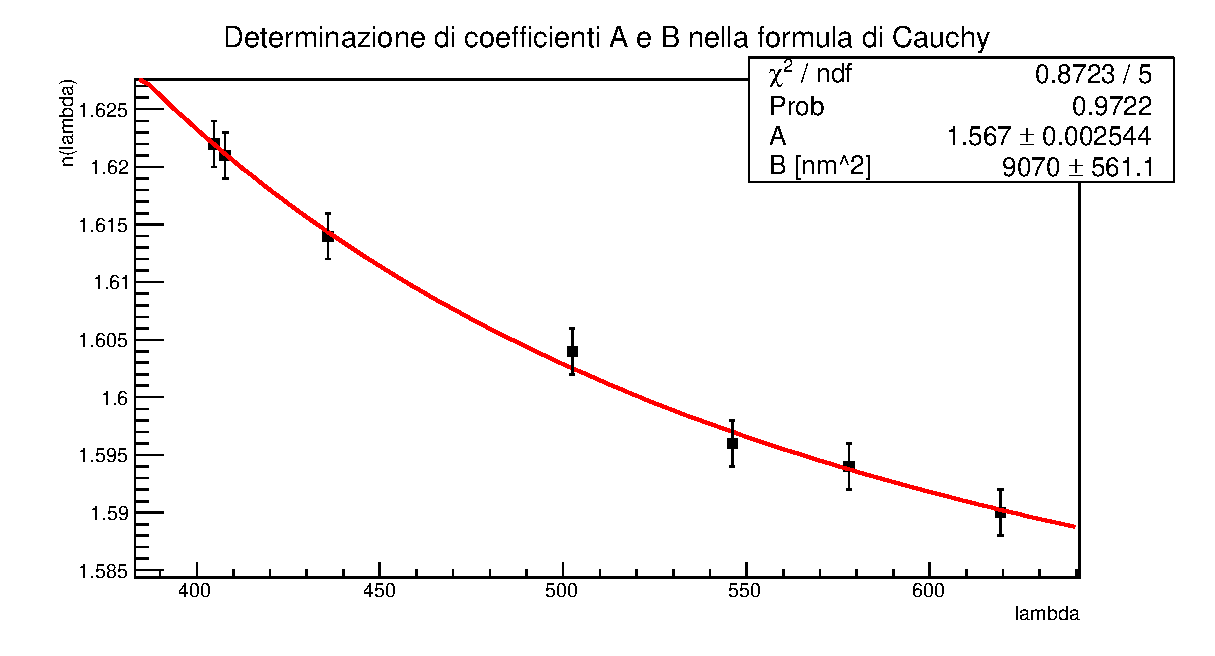
\includegraphics[scale=0.8]{Grafici/O3_P2_1_AB.eps}
    %\caption{}
    \label{fig:C3_P2_RL}
    \caption{Verifica legge di Cauchy. Fit: $y = [0] + [1]/x^{2}$ dove $y = n$, $x = \lambda$, e i parametri da stimare $[0] = A$ e $[1] = B$. }
    \end{figure} 
%
%
%
%
Coefficienti della formula di Cauchy stimati dal fit:
$$ A = 1.567 \pm 0.003 \quad ;\quad B = 9100 \pm 600 \;\mathrm{ nm^{2}} $$
%
\paragraph{Osservazioni:}{ Il $\chi^2$ risulta troppo basso. Si sospetta una sovrastima degli errori. Si applica il procedimento della stima dell'errore a posteriori come descritto nel paragrafo \ref{sec:C3_final}
%reference:Paragrafi/C3_finale.tex
Di seguito il risultato del nuovo fit.

    \begin{figure}[H]
    \centering
    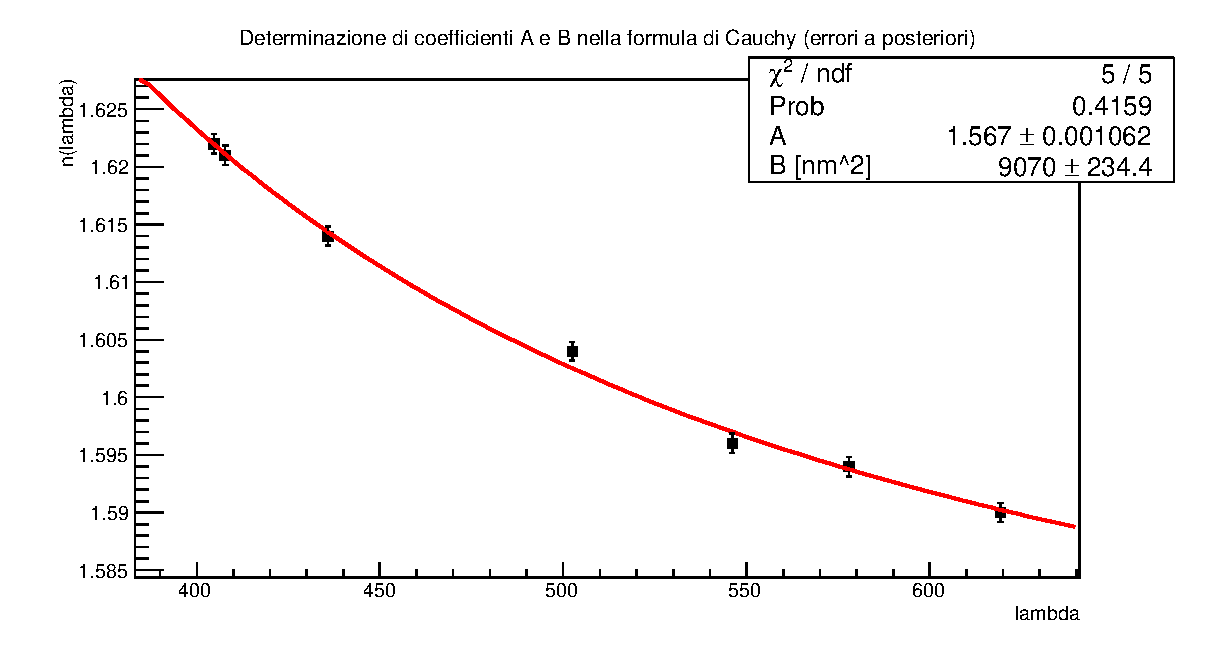
\includegraphics[scale=0.8]{Grafici/O3_P2_1_AB_p.eps}
    %\caption{}
    \label{fig:C3_P2_RL}
    \caption{Verifica legge di Cauchy con errori stimati a posteriori. Fit: $y = [0] + [1]/x^{2}$  }
    \end{figure}
%
%
Da questo nuovo fit si ottiene:
$$ A = 1.567 \pm 0.001 \quad ; \quad B = 9100 \pm 200 \;\mathrm{ nm^{2}} $$
che vengono assunti come stima di A e B.    
}  
